
\graphicspath{ {mainmatter/Omodhrain_2004/} }

\title*{2004: PebbleBox and CrumbleBag: Tactile Interfaces for Granular Synthesis}
\titlerunning{Tactile Interfaces for Granular Synthesis}

\author{Sile O'Modhrain and Georg Essl}
\authorrunning{O'Modhrain and Essl}


%\institute{Sile O'Modhrain \at Media Lab Europe, Sugar House Lane, Dublin 8, Ireland \email{sile@media.mit.edu}
%\and Georg Essl \at Media Lab Europe, Sugar House Lane, Dublin 8, Ireland, \email{georg@mle.media.mit.edu}
%}
%
%
\maketitle

\abstract*{The PebbleBox and the CrumbleBag are examples of a granular interaction paradigm, in which the manipulation of physical grains of arbitrary material becomes the basis for interacting with granular sound synthesis models.  The sounds made by the grains as they are manipulated are analysed, and parameters such as grain rate, grain amplitude and grain density are extracted.  These parameters are then used to control the granulation of arbitrary sound samples in real time.  In this way, a direct link is made between the haptic sensation of interacting with grains and the control of granular sounds.}

\section{Introduction}

Interaction with objects in the world around us is a richly multisensory experience.  Casting a pebble into a pond, we both see the ripples resulting from the disturbance of the water's surface and hear the impact of the stone on the water as a disturbance of the air.  If we are close enough and the stone is big enough, we might also get wet.  Furthermore, the interaction of stone and water makes certain information explicit---the size of the splash is correlated with both the size of the stone and the force with which it was thrown, and the sound it makes provides information about the depth of the water.  Thus the physical laws that govern the behaviour of stones falling into water give rise to an event which is perceived via many sensory channels which each encode, in their different ways the complexity of the event.  The perceptual system therefore has a number of representations of the event upon which to draw.  In this paper, we suggest that it is possible to build a methodology for sound control upon commonalities between the behaviour of physical objects and that of sound objects which share many of their physical properties.  In particular, we focus on the technique of granulation, presenting two instances of expressive instruments for live control of granular 
synthesis. 

Granular synthesis has long been an important and widely used compositional technique in Computer Music. Its literature is too extensive to be sufficiently reviewed here---we refer the reader to a recent comprehensive exposition by Curtis Road \cite{Roads:2001}.

Granular synthesis has also been used in live computer music performance including novel interfaces for expressive control of granulated sound. For example, in ``The Lobster Quadrille'' \cite{Trueman:1999a}, Dan Trueman used his sensor-augmented violin bow, (the RBow \cite{Trueman:1999}), to play granular models. Additionally a number of controllers related to granular synthesis have been proposed. These include Timothy Opie's Fish \cite{Opie:2002,Opie:2003} Gadd and Fels' MetaMUSE \cite{Gadd:2002}, Perry Cook's PhISM and FoleyMat controllers \cite{Cook:1999b,Cook:2002} and the MIDI keyboard and laptop based Creatovox by Roads  \cite{Roads:2001}. Cook also proposed a granular approach to Gait synthesis \cite{Cook:2002} which is also related to other footware controllers \cite{Paradiso:1997a}.  While all of these controllers drive granular synthesis, and have some haptic feel to them, they usually do not retain the haptic component of the granular interaction itself. For example, Cook's PhISM shakers retain the form factor and weight of an acoustic shaker, but the moving particles (pebbles or the like) are removed and replaced by rigidly anchored electronics. Hence the performer does not feel the particle interaction---they feel the coarse haptic experience but not the fine detail. This also holds for Gadd and Fels' MetaMUSE \cite{Gadd:2002} and the RBow \cite{Trueman:1999}. In the case of the Opie and Road's controllers, the control gesture is abstracted from the interaction and neither level is captured directly.

Our interest here is in retaining the haptic features that are relevant for the parametric control of the sound synthesis algorithm.  To the best of our knowledge, this goal has not been explicitly stated elsewhere in the literature.  While musical devices that have implicit haptic components have been explored elsewhere e.g. the Musical Playpen and Musical Candy Bowl of  Weinberg and coworkers \cite{Weinberg:1999,Weinberg:1999a} which employed spatially distributed accelerometers, these were not used for tight musical
coupling or control of event-based granular synthesis. 

\section{Design Goals}

The overarching goal of our work on haptic controllers for computer-based musical instruments is to uncover instances of coupling, however loose, between the haptic and auditory senses and to build on these couplings to develop new paradigms for instrument control. The examples presented here represent a sub-set of such controllers, those based on interactions that are mediated by physical objects,the properties they embody and the manipulation strategies they invoke.

For more details on experimental investigations into the importance of haptic feedback for musical performance see \cite{OModhrain:2000}).

Since the current goal was to build a controller that couples the feel and sound of granular events, it was  important  to incorporate into the interface the manipulation of elements that could objectively or subjectively give rise to granular sounds.  Two different interaction paradigms were developed, playing with a hand-full of pebbles and crushing a bag of brittle material. Both are somewhat complex environmental events, whose temporal patterns give rise to important perceptual cues \cite{Keller:2001,Warren:1984}.

Therefore, there is a need to sense these temporal events. This poses a number of problems. Firstly, given the nature of the sounds of interest, the events are likely to be spatially distributed. Moreover, the sound-producing mechanism may be internal to the objects interacted with crinkling paper,or may be a result of their destruction (for example crushing cornflakes.)

Finally, while the coupling between temporal events as they are perceived by both the haptic  and auditory system should be relatively tight, we are interested in leaving other parameters such as dynamics and timbre open for exploration by the performer.

\section{Controller Design}

At the heart of our design of haptic controllers for granulated sounds is a recognition that there exist a class of sounds which are produced by our actions on objects in the world.  Thus dragging, dropping, scraping and crushing give rise to to correlated touch and sound events \cite{:2003b}.  As noted earlier, such events also bear many signatures of other physical characteristics  of the materials and actions involved.  However, it is possible to imagine a further class of events where the feel of an object and the sound it produces are less strongly correlated---for example, when playing with pebbles in ones hand, the haptic sensation one feels is that of the pebbles against the hand, while the sound of the interaction stems from the colliding of pebbles within the hand.  This loose correlation between feel and sound is appropriate for this experience and in its looseness provides an opportunity to decouple the haptic experience from the sound source.  This is the opportunity we build on in our granular synthesis controllers.  The first example, the Pebble Box, is based on the manipulation of objects in the environment---the manipulation of pebbles in a tray.  The second, the Crumble Bag, is based on the manipulation of an ensemble of grains contained in a malleable skin.

%\vfill
\subsection{Object Interaction: PebbleBox}

The PebbleBox is designed to allow for direct manipulation and 
ecological behavior of objects in a relatively unconstrained way. See Figure~\ref{Omodhrain:fig:pebblebox}.

\begin{figure}[t]
\centering
%\epsfig{file=PebbleBoxWins.eps,width=\columnwidth}
%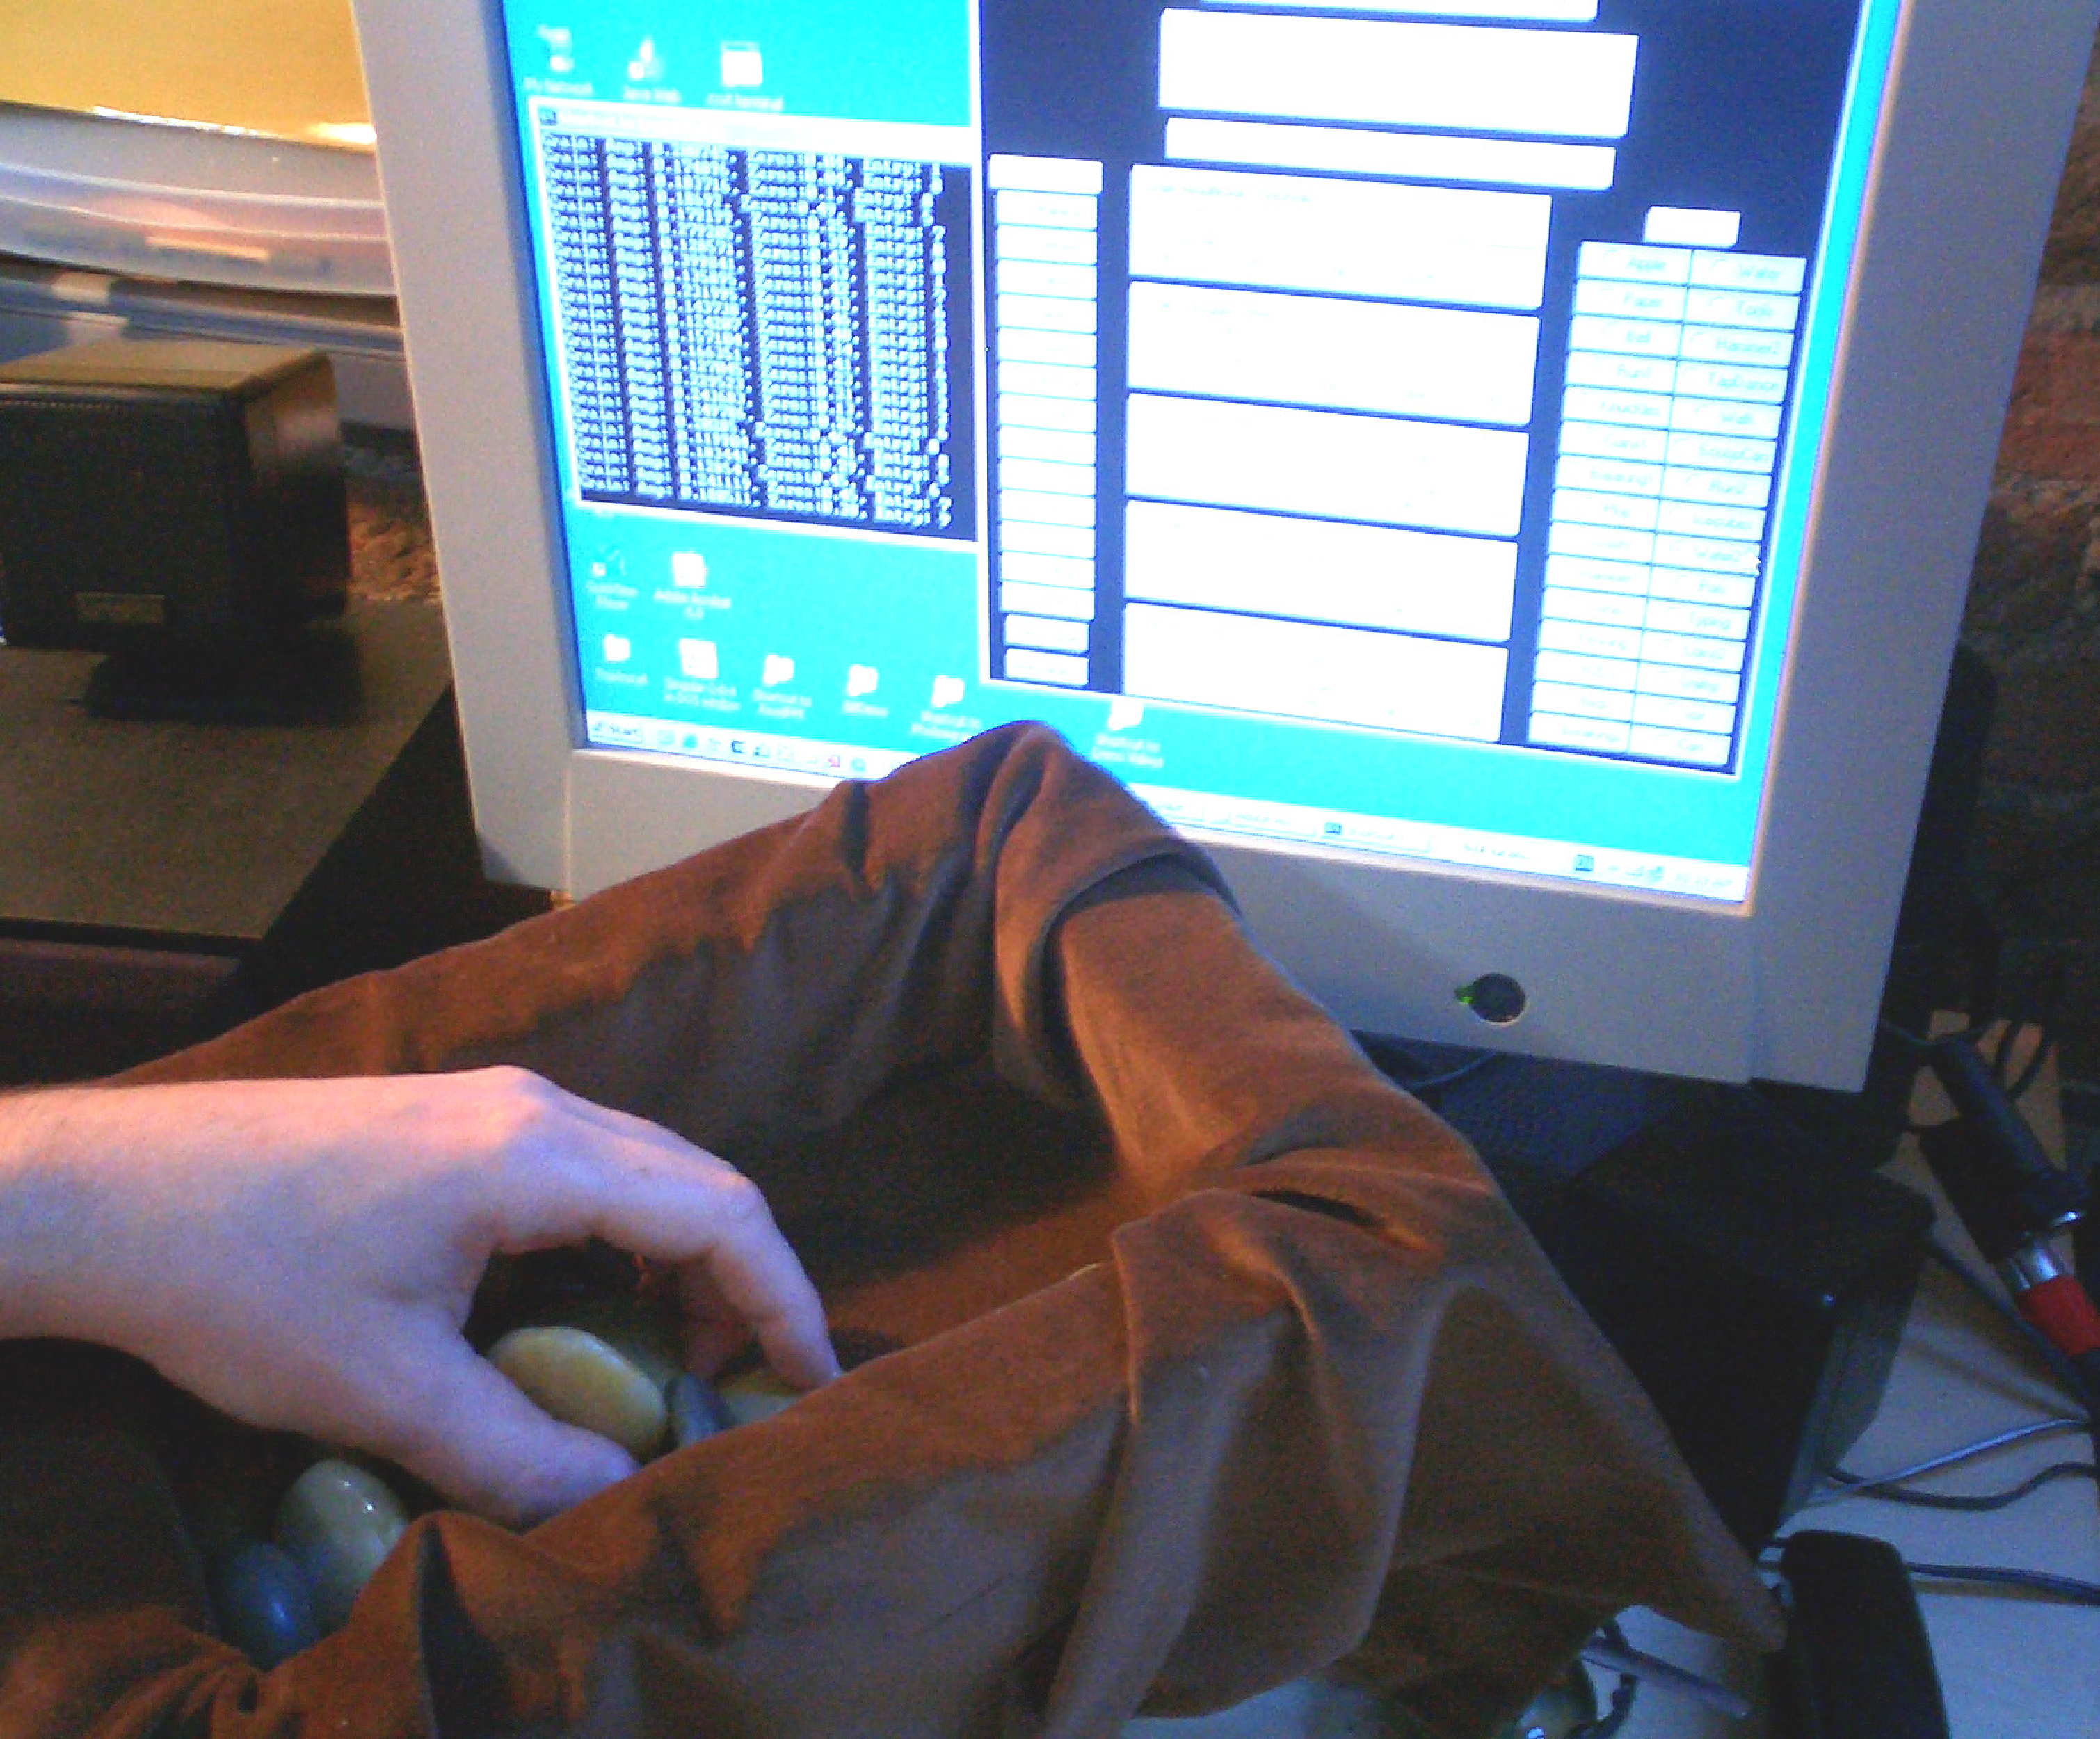
\epsfig{file=pebblebox-new-cropped2-eps-converted-to.pdf,width=\columnwidth}
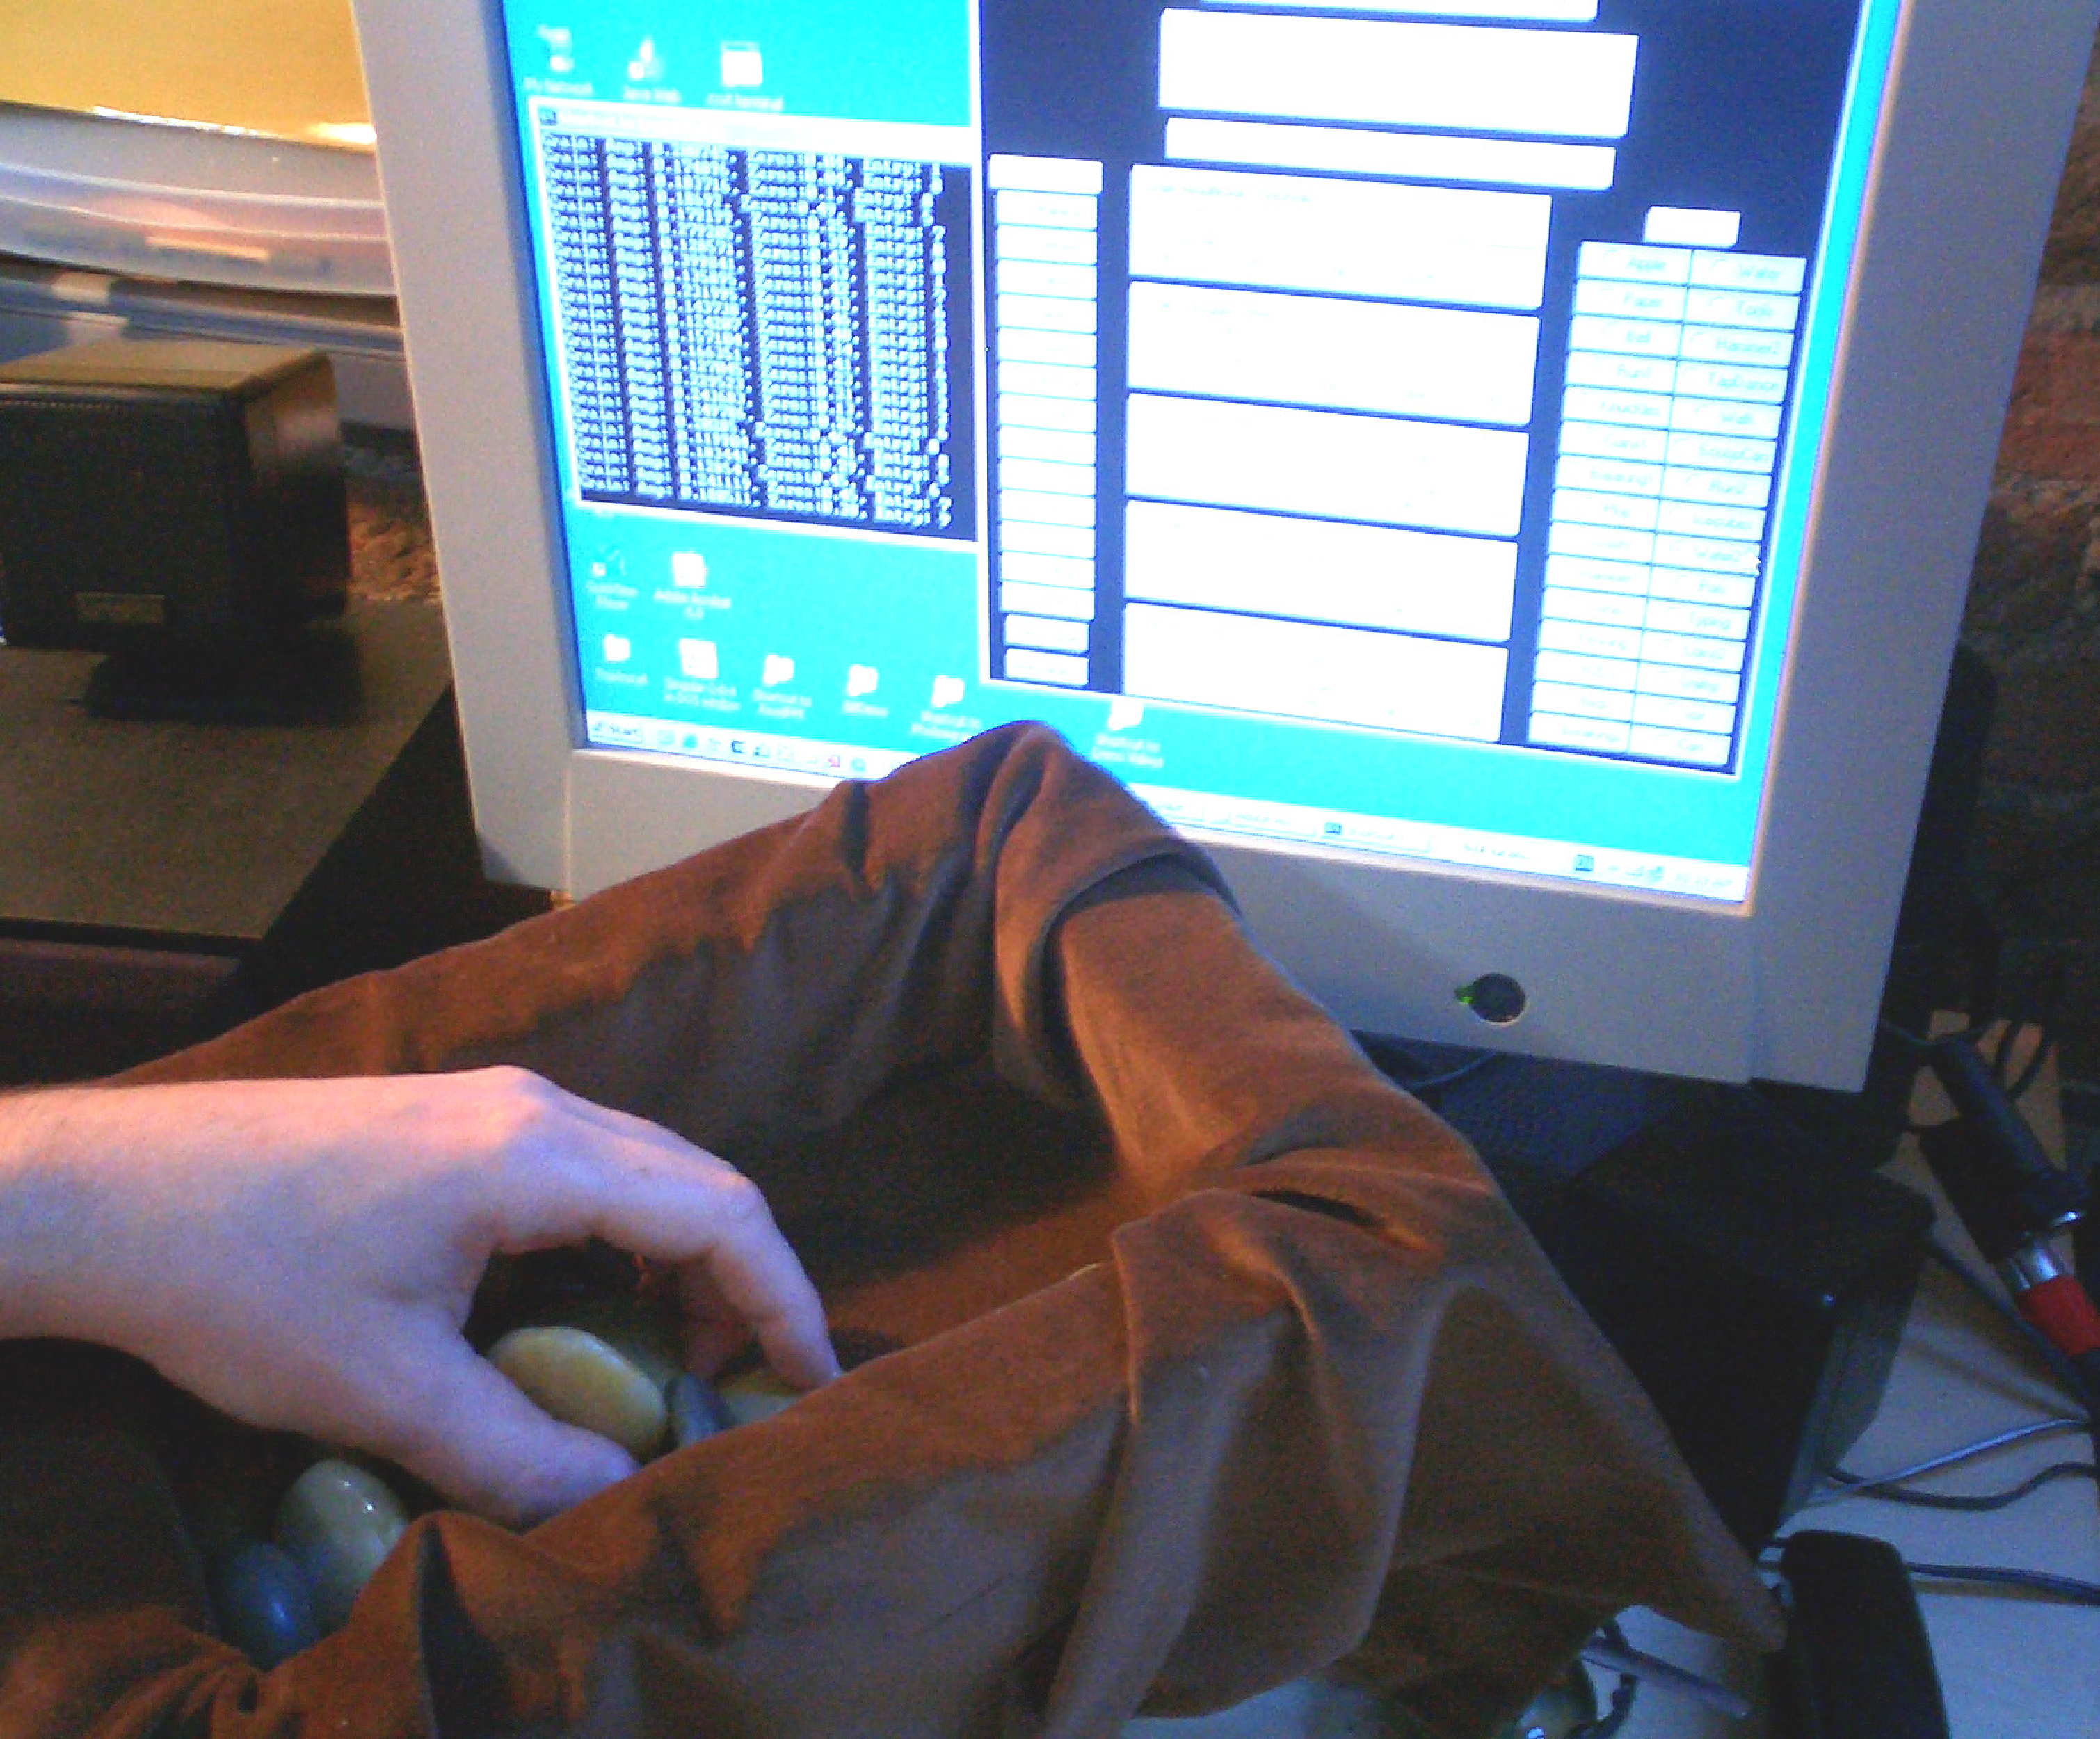
\includegraphics[width=90mm]{pebblebox-new-cropped2-eps-converted-to.pdf}
\caption{The PebbleBox.}
\label{Omodhrain:fig:pebblebox}
\end{figure}

\begin{figure}[t]
\centering
%\epsfig{file=Mic-trimmed2s.eps,width=\columnwidth}
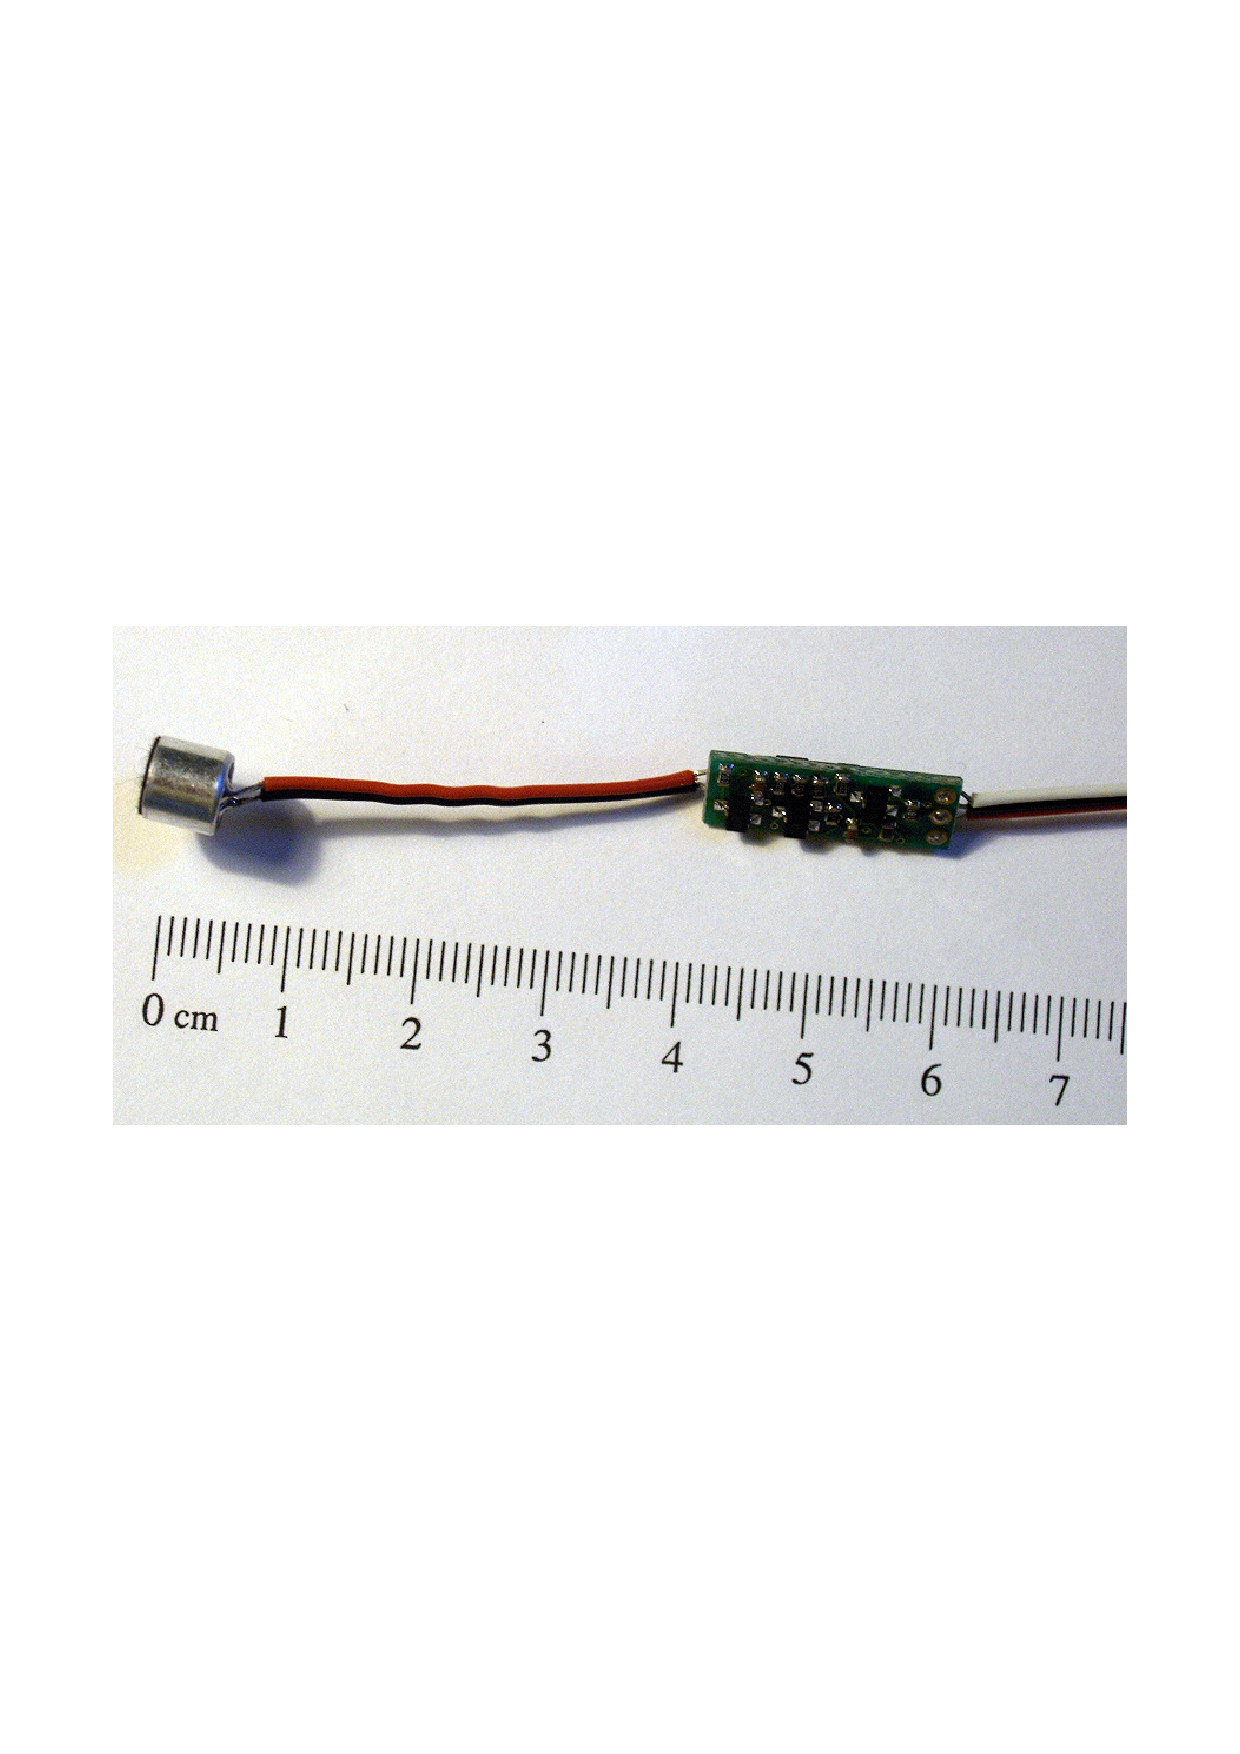
\includegraphics[width=90mm]{Mic-trimmed2s-eps-converted-to.pdf}
\caption{Microphone used for both devices.}
\label{Omodhrain:fig:mic}
\end{figure}

The design consists of a foam-padded table with an in-laid actively
powered microphone (see Figure~\ref{Omodhrain:fig:mic}). The purpose of the foam
is to eliminate the possibility of objects colliding with the container and to damp the sounds of objects dropped or rolled inside the
box. However, interactions and disturbances are still picked up by the
embedded microphone.  Additionally, the microphone picks up
interactions in a limited range above the device, i.e. the interaction of objects held in the hands just above the box.

Typical sounds are the collision of objects with the foam padding
and collisions between objects.

Haptic feedback is a result of the direct manipulation of
the objects in the PebbleBox. The flexibility of this approach allows for the manipulation of any collection of small objects---we have experimented with polished stones, ball bearings and crumbling paper. Each material suggests its own gestures: grabbing, dropping, tapping, crumbling, shuffling,
rolling and so forth.

\subsection{Grabbing Action: CrumbleBag}

The {\em CrumbleBag} is a flexible bag made of neoprene, into which different granular materials can be placed. The concept, it is derived from the
sand-bags used by traditional Foley artists. Through the use of grabbing gestures, the
artist articulates foot-steps and the material used in the bag defines
the property of the material that is being stepped on (for example
corn flakes for leaves and cornstarch for snow \cite{Ebersole:2003}).

\begin{figure}[t]
\centering
%\epsfig{file=CrumbleBags.eps,width=\columnwidth}
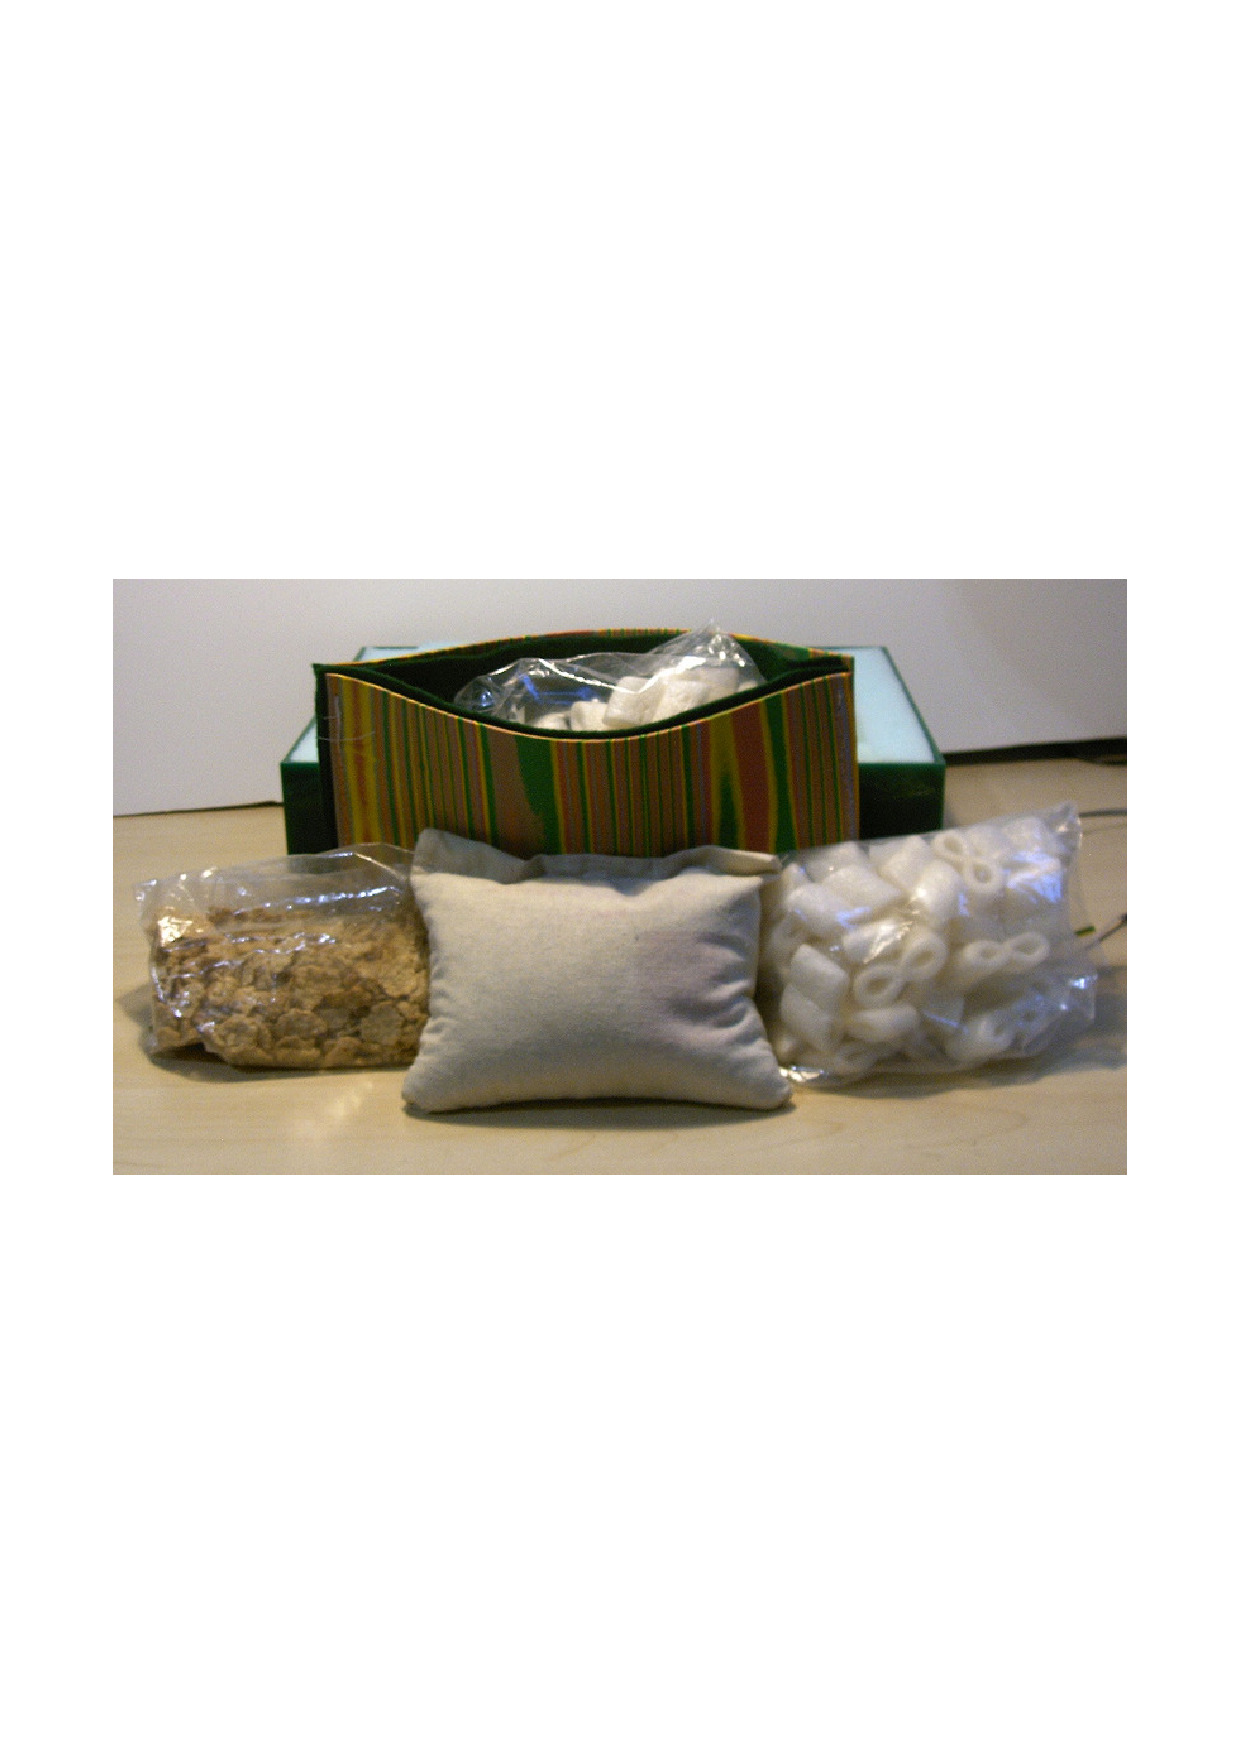
\includegraphics[width=90mm]{CrumbleBags-eps-converted-to.pdf}
\caption{The CrumbleBag with cereal, coral and Styrofoam fillings.}
\label{Omodhrain:fig:crumblebag}
\end{figure}

So far, we have experimented with corn-flakes and ground coral (in plastic and cloth lining bags), Styrofoam beads, and a metallic chain as filling examples, each yielding a very different set of dynamic control parameters (See Figure~\ref{Omodhrain:fig:crumblebag}.)


\begin{figure}[t]
\centering
%\epsfig{file=FoamPlot.eps,width=\columnwidth}
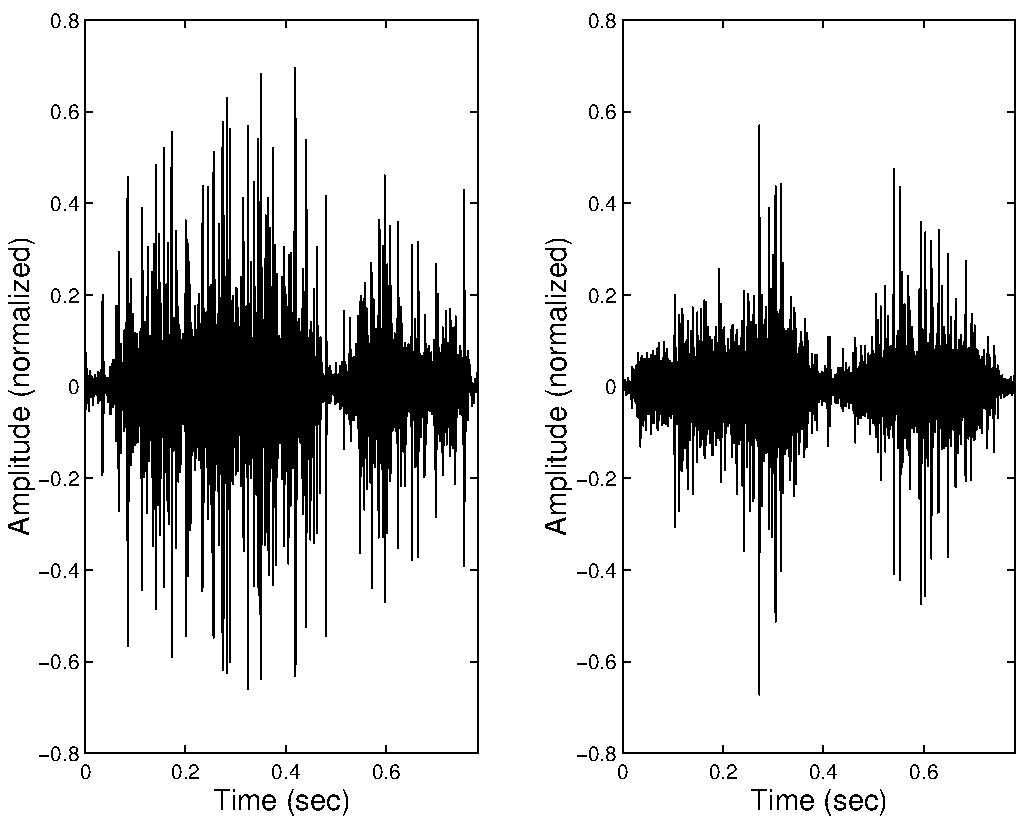
\includegraphics[width=90mm]{FoamPlot-eps-converted-to.pdf}
\caption{Grabbing of the CrumbleBag with Styrofoam filling in a plastic bag (left) and a cloth bag (right).}
\label{Omodhrain:fig:styrocomp}
\end{figure}

Figure~\ref{Omodhrain:fig:styrocomp} compares the effect of plastic bag versus
cloth bag. The recorded instance is one grabbing event. The cloth
sound is more muffled whereas the noise created by the plastic adds
somewhat to the plastic bag sound, notice however the overall
similarity of grain envelope and temporal progression.

Haptic components of the interaction can still be felt through the bag. For example the
breaking of cereal or the shifting of coral sand will be felt and the
material resistance is maintained.

\section{Audio-Driven Granular Synthesis}

Live audio based sound manipulation is a known
concept. It has for instance been used by Jehan, Machover and
coworkers \cite{Jehan:2001a, Jehan:2002}, though in their case the relationship between audio event and
haptic action was not explicitly retained, as the
audio was driven by an ensemble mix of traditional acoustical musical
instruments as opposed to single instrument granular events.

Granular processing is usually related to what Lippe called ``Granular
Sampling'' \cite{Lippe:1994} but can also be Wavelet inspired processing
\cite[offers a review]{Roads:2001}. Neither of these processing
paradigms adequately captures the properties we require for intimate interactive
control and hence we draw from music, speech and sound retrieval literature
for ideas to arrive at practical real-time ``granular analysis''
algorithms that allow for the grain-level control, that we are looking
for.

\subsection{Grainification Process}

To use the raw audio signal as a driver for granular synthesis, the
signal stream needs to be analyzed for granular events. This procedure
is somewhat different from granular sampling and we will call it {\em
grainification}. It does, however, relate to event detection as described by
Puckette \cite{Puckette:2003}.

The parameters that we considered desirable were event detection in the
temporal range of perception ($>.1 s$), an amplitude measure of a
granular event and a measure of spectral content.

The procedure is constrained by the real-time nature of the design
goal. Firstly, we are bound by causality and hence any consideration
for oncoming data translates into delay. Also the amount of processing
is bound by the playback buffer length, which in turn translates into
delay. 

\begin{figure}[t]
\centering
%\epsfig{file=GrainThres4.eps,width=\columnwidth}
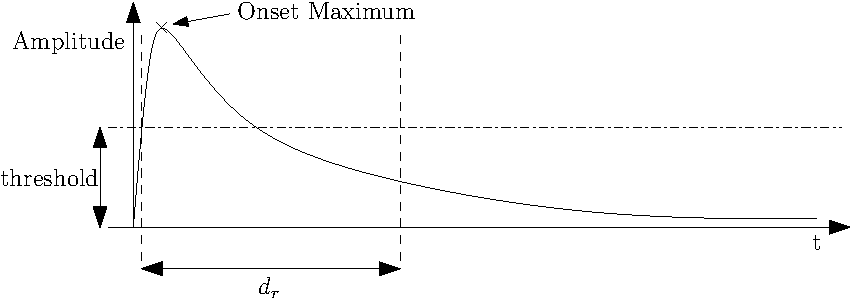
\includegraphics[width=\textwidth]{GrainThres4-eps-converted-to.pdf}
\caption{Threshold based grainification scheme. The curve displays an amplitude envelope of an event. $d_r$ is the retrigger delay, preventing detection of new onsets.}\label{Omodhrain:fig:grainenv}
\end{figure}

Given these constraints we employ the following procedure in the
current prototype: A very basic onset and retrigger prevention
algorithm which also includes a moving short-time average
zero-crossing average. The onsets are detected by thresholding
followed by a local maximum detection. We do not employ averaging for
envelope as we assume that the events have impulsive onsets, hence the
first gradient should be expected to  lead to a strongest
maximum. This amplitude is then used as an immediate measure of grain
strength. After a grain event is detected, the detection for further
granular events is postponed until  a certain time has expired
(a so-called retriggering delay $d_r$). The purpose is to detect only
events that lie in the temporal range of perception ($t>0.05-0.1 s$ 
or alternatively $f<10-20Hz$). The second purpose of this procedure is
to avoid spurious retriggering by the decaying oscillation of the
detected grain, waiting until  the grain has decayed below the
detection threshold. Hence the inherent signal assumptions are rapid
onset, decaying envelope events, where the decay is of the order of
the retriggering delay $d_r$ or faster. For this reason this procedure would not
be meaningful for the class of sustained sounds which
would  be inherently less suited to the type of temporal pattern  that
we are trying to extract. The relationship of thresholding and retrigger delay to a grain amplitude envelope can be seen in Figure~\ref{Omodhrain:fig:grainenv}. The final measure we employ is moving average
zero-crossing count. Over a short-time moving window, the number of
zero crossings are calculated. This value is used as a spectral
measure. The number of zero-crossing is bound from below by the lowest
present frequency in a signal \cite{Eremenko:2003} and has a correspondence
overall with the dominant spectral content of a signal (i.e. the
spectral centroid) \cite{Panagiotakis:2004,Peeters:2002}.

\begin{figure}[t]
\centering
%\epsfig{file=PebbleSpecPlot.eps,width=\columnwidth}
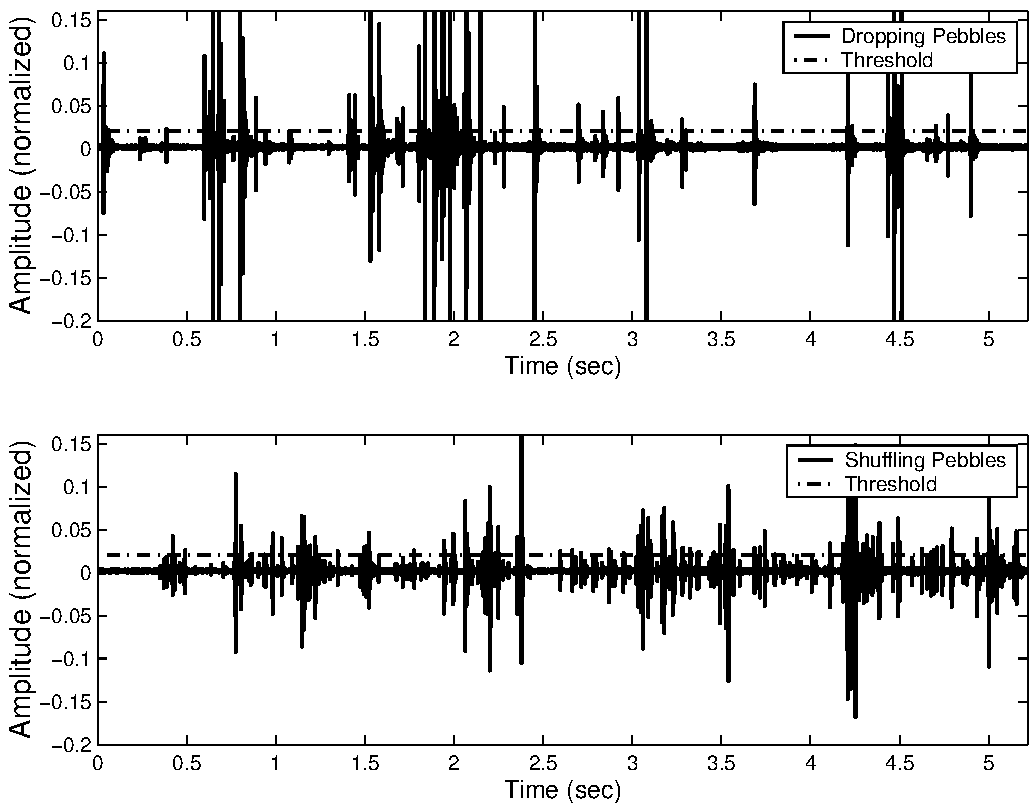
\includegraphics[width=\textwidth]{PebbleSpecPlot-eps-converted-to.pdf}
\caption{Thresholding of dropping pebbles (top) and pebbles shuffled in one hand (bottom).}
\label{Omodhrain:fig:dropgrab}
\end{figure}

We found that despite these assumptions and the simplicity of
implementation of this procedure reliable grain detection and
believable control is achieved and hence more advanced methods were
not concerned. Figure~\ref{Omodhrain:fig:dropgrab} shows two audio signals as
detected, including the threshold. The first signal shows pebbles
being dropped into the PebbleBox and the second displays a handful of
pebbles being shuffled in the player's hand above the pebble box. As
can be seen the dropping are more distinctly temporally separated
events, whereas the shuffling creates a denser pattern. As can be seen
the impulsive assumption of the signal as well observed, and grains
are well-separated from background noise.

The real-time implementation is based on STK's real-time audio
duplexing. We found an input and output buffer size of $128$ to work
without clicks or missed buffers. This buffer size, at $22050 Hz$ corresponds to a
basic delay of $11.6 ms$. Typically grain estimation windows of $100$
samples were used leading to a total delay of around $16.1
ms$. Performance measures are taken on a $1.6GHz$ Pentium 4 PC
 running Windows XP with 256 MB ram and a SoundMAX Integrated
Digital Audio device by Analog Devices.
%,
%which lies within the range of transition to undetectable offset
%asynchrony of $10-30ms$ \cite[p. 173]{Moore:1997}.

%Onset detection \cite{HM03}. Onset intensity and spectral
%content. Zero-crossing and spectral centroid \cite{PX02,PT04} for mathematical aspects see also \cite{EN03,Arnold02}.

%\subsection{Haptification and Haptic Authoring}


\section{Examples and Applications}

%\subsection{Mapping}

To test the controller in a real application, the extracted data needs to be
mapped to sound generation mechanisms. This is the \textit{mapping
problem}, which has seen both theoretical and experimental advances
\cite[for example]{Hunt:2000b,Hunt:2002,Rovan:1997}.

In principle the sensed data can be mapped arbitrarily. Here we
consider the application of our controller design to two types of granular synthesis. The first is
based on recorded dictionaries of environmental sounds. The second
uses parametric physically informed models developed by Perry Cook
 \cite{Cook:1997,Cook:1999b,Cook:2002}. 

\subsection{Recorded Environmental Sound Grains}

We implemented a prototype grain dictionary based on recordings of
natural sounds. 30 grains were explored using between one and 12
recordings of comparable events. More recordings were used when similar
interactions led to different sonic experiences, as for example water
splashing or the buckling of a can, or where the detail of the
interaction is hard to control and hence leads to variation as in the
case of walking, or the shuffling of coins.

The grains are played back based on the granular parameters in the
grainification process. The onset time triggers a variable playback
event with the playback amplitude defined by the grain onset
amplitude. The playback rate, as a measure of the grains overall
frequency, was varied with the average zero crossing at the instance
of onset. In the absence of the last procedure, the sound is
repetitive and multiple entries in the dictionary of similar grain
instances are necessary. Three grains are found to be still too likely
to have consecutive instances of equal sound events, whereas this was
improved with 8 grains. In the presence of variable frequency the
monotonous appearance of the sound disappears even for only one
recorded grain. In the case of multiple grain recordings for one grain
event in the dictionary, a particular instance is chosen at
random. The relationship between recorded collision sounds and final
sound using a Hammer grain using the PebbleBox can be seen in Figure
\ref{Omodhrain:fig:compspec}.

\begin{figure}[t]
\centering
%\epsfig{file=CompSpecPlotBW.eps,width=\columnwidth}
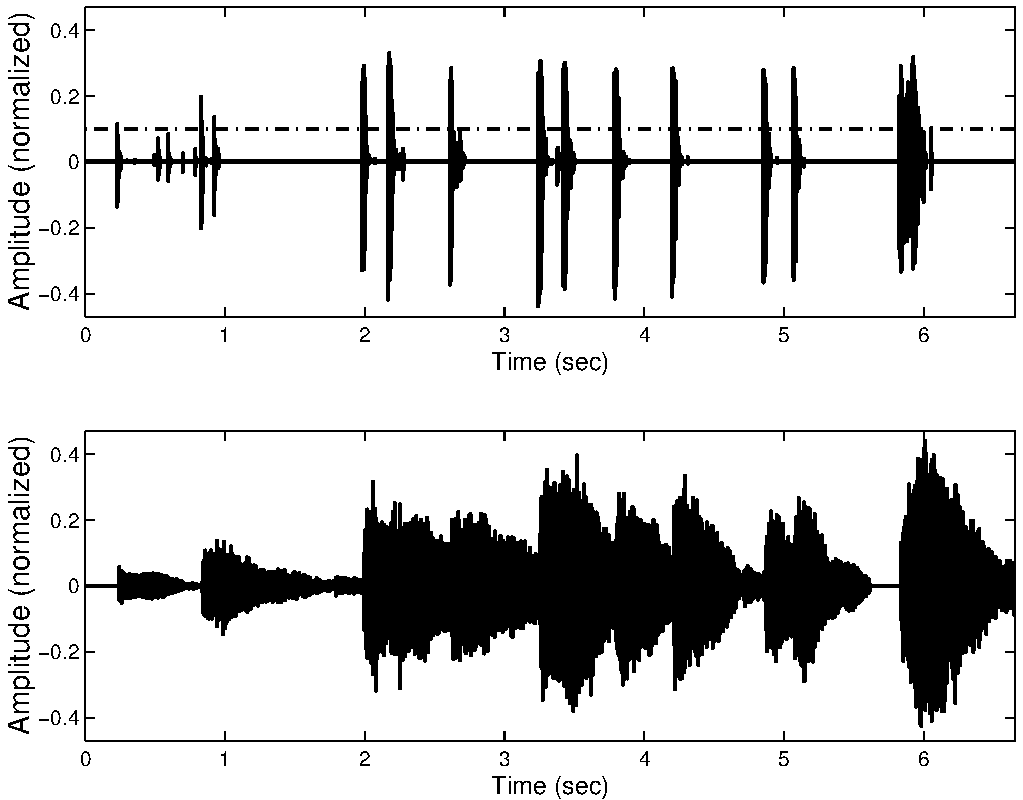
\includegraphics[width=\textwidth]{CompSpecPlotBW-eps-converted-to.pdf}
\caption{Recorded signal of the PebbleBox (top) and granulated response using a Hammer grain (bottom) of the complete granulation process.}
\label{Omodhrain:fig:compspec}
\end{figure}

\subsection{Physically Informed Parametric Models}

In order to explore parametric models, we used Perry Cook's shaker
based granular synthesis as implemented in his STK software
 \cite{Cook:2002}(see the left button row in Figure~\ref{Omodhrain:fig:stkgui}).

Here the mapping of grain onset time and amplitude relates to time and
amount of energy infused into the physically inspired model. The
zero-crossing average is mapped to the center resonance frequency of
the models. These models have inherent stochastic variability. Also
some do respond more immediately to energy infusion than others. This
does affect the perception of playability, and in general a strong
correlation of energy infusion to granular events is desirable. For
details on the parametric model synthesis we refer the reader to
 \cite{Cook:1997,Cook:1999b,Cook:2002}.

\begin{figure}[t]
\centering
%\epsfig{file=STKWindow3f.eps,width=\columnwidth,}
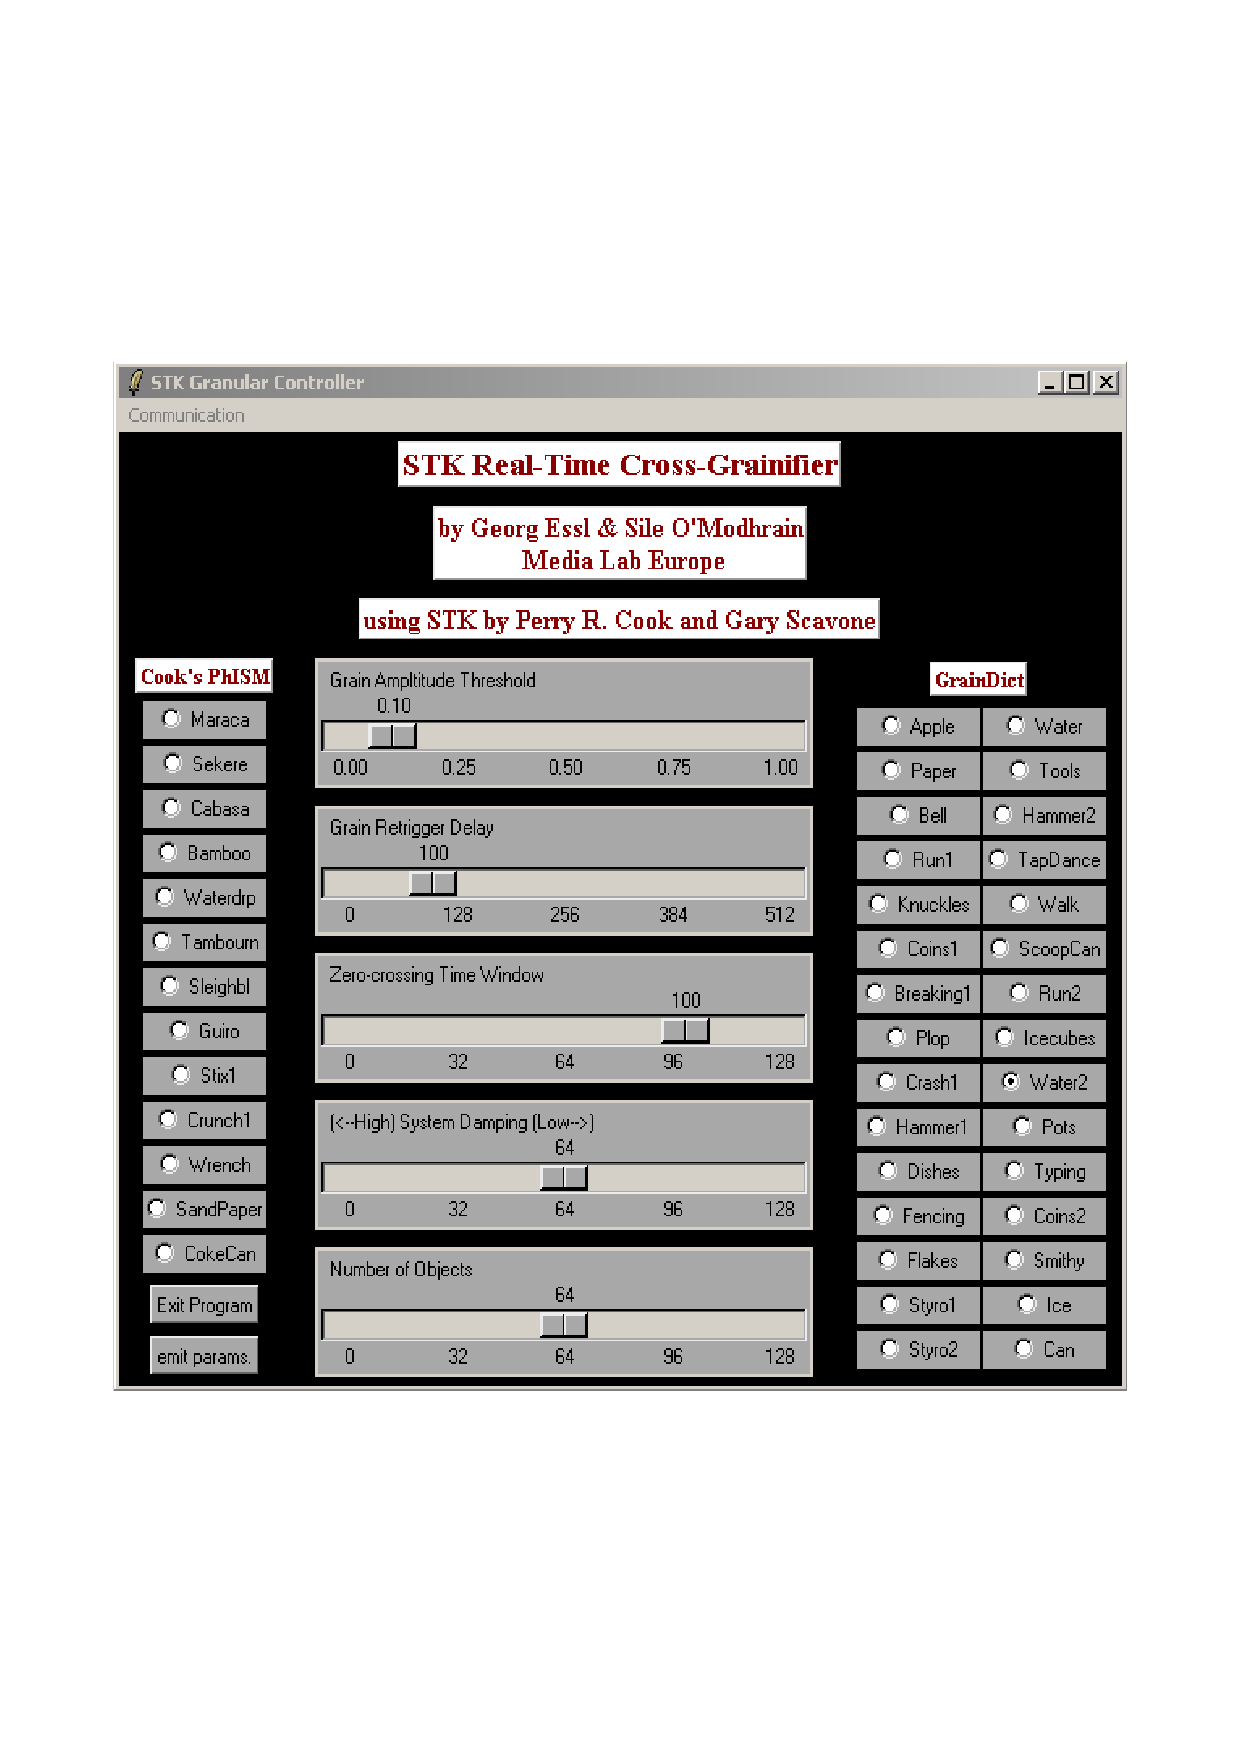
\includegraphics[width=\textwidth]{STKWindow3f-eps-converted-to.pdf}
\caption{The interface of the Grainification and Synthesis Application GUI implemented in STK.}
\label{Omodhrain:fig:stkgui}
\end{figure}

%\subsection{Abstract Parametric Models}

%\begin{figure}[t]
%\centering
%\epsfig{file=HaptoGrinder2.eps,width=\columnwidth,}
%\caption{The interface of the Haptio-Sonic Schmeister.}
%\end{figure}

\vfill
\section{Conclusion}

The advantage of the proposed design is its simplicity and low cost, and the flexibility which supports the exchange of interaction materials for varied haptic performance experiences and spectral control over the granular synthesis process. Drawbacks include the possibility of environmental noise that could interfere with the performance. In practice, however, we found that ongoing background conversation and extraneous sounds in a large shared office space  did not affect the performance of the device unless the speaker were in the immediate vicinity of the device. Another drawback of the current design is the lack of spatial information, a drawback that might be overcome by multiple channel microphone recordings at various positions inside the PebbleBox or the CrumbleBag. Finally only basic granular features are currently extracted and additional degrees of freedom may be desirable.

To our knowledge, this is the first controller for granular synthesis which maintains the individual mapping of fine-structure temporal behavior of the order of 10--100ms of granular event to haptic interactions, while not having the haptic interaction abstracted from the expected sounding mechanism. In the particular implementation of onset grains, the mapping is flexible, but remains intuitive for sounds that have comparable temporal patterns to the recorded sounds. The haptic feel of the instrument  is modular and can be adjusted by exchanging interacting objects, in the case of the PebbleBox, and by varying filling materials, in the case of the CrumbleBag. In this way a variety of environmentally based sounds, like dropping or shuffling of objects can be performed. Also imitated gestures such as walking can be controlled by enacting the characteristic time patterns of sounds. Furthermore, the opportunity exists to create new abstract sounds by imposing unconventional temporal patterns, which don't mimic the behaviour of these environmental sounds.

In summary, we have presented an environmentally based haptic controller which maintains the  feel of physical granular processes and allows for real-time performance of granular synthesis methods.

\begin{acknowledgement}
We would like to thank Erin Panttaja for providing sowing material. Andy Brady for much help with material and design. Stephen Hughes for many helpful suggestions. Best thanks to Martin Kaltenbrunner for kindly providing his digital camera. Erik Blankinship for pointing out relevant references. Michael Bennett for enlightening discussions. Also much thanks to Simon Jones for pointing out a relationship of this work to TEMPEST.\footnote{\url{http://fas.org/irp/program/security/tempest.htm}}
\end{acknowledgement}

\section*{Author commentary: ``PebbleBox and CrumbleBag'': 12 years later}
\paragraph{Sile O'Modhrain and Georg Essl}

When we wrote this paper, one of the central research questions in musical instrument design was the question of how to  define the relationship between musical gestures and perceptual (musical) outcomes. This remains a significant problem today. Without further information, the number of possible mappings is seemingly endless and requires the players to ``discover'' meaningful relationships between their actions and an instrument's response.  PebbleBox and CrumbleBag proposed that both ecologically relevant and cognitive aspects of an interaction can be used to inform the process by which such relationships are discoverable.  In our work, we took as a starting point an established method of synthesis with some potential ecological grounding, namely granular synthesis, and conceived of interfaces that provide what one might call ``natural'' mappings between controller actions and synthesis results. 

An important component in the design of Pebblebox and CrumbleBag revolves around exploiting cognitive phenomena and capabilities in their design. While the stones in PebbleBox are not replaced, the sounds that are triggered by their collisions can be changed. For a number of sounds, we found that this maintains a credible interaction. Coins, blades, and even water all led to quite believable perceptual qualities, while other sounds such as cats meowing or people biting apples are less credible sonic outcomes for typical stone collision interactions. How sounds cluster cognitively with respect to different gestures is still a wide open research question. In our own work we looked to quantify this perceptual malleability through the notion of ``believeability'' \cite{Essl:2005}. 

While perception and cognition played a role in the original design idea behind these interfaces, the thinking in this direction became much more clearly defined in the following years. Multi-sensory integration and the role of the relationship between action and perception (the relationship captured by the word ``enaction'') became a topic of strong theoretical interest, and offered a new perspective on the guiding research questions that feed into instrument design. 

The underlying question posed here can be framed very generally as: ``How are musical instruments perceived?'' This question not only encompasses sonic and musical perception but also a more complete perception of the instrument's physicality, including motor action, tactile feedback, and visual feedback, as well as cognitive aspects such as prior experience. In this sense, PebbleBox and Crumblebag  prefigured a kind of cognitive/perceptual perspective in thinking about new musical instrument design. Enaction is a cognitive theoretical framework that emphasizes the idea that action guides perception which in turn guides future action.  Hence, it is not surprising that a number of researchers have embraced this approach in subsequent instrument designs.  Our own expanded thinking that was anchored in iterations of PebbleBox appeared two years later \cite{Essl:2006}. Around the same time, Newton Armstrong published a Ph.D. thesis engaging with the topic \cite{Armstrong:2006} and David Wessel published a paper developing related concepts \cite{Wessel:2006}. 

In many ways, PebbleBox and CrumbleBag were just first steps in this direction since, in their design, they focused on grain-based interactions. A later project called ``Scrubber'' looked to expand this direction toward friction-based interactions. And clearly there are many other possible ecologically-founded phenomena that remain unexplored, and an associated cognitive taxonomy of perceptional grouping of sounding phenomena with respect to motor actions and tactile perceptions still needs to be fully developed. We believe that studying the perception of musical instruments and exploiting perceptual and cognitive phenomena in instrument design remain important research topics. There is much we do not yet understand about either. This kind of work is particularly interesting, not only to those seeking to develop new musical instrument designs but also as a critical component in applications where musical instruments interface with other fields of endeavor.  An early example was developed by Young, Roger, and Craig, who studied cross-sensory integration in Parkinson's patients \cite{Young:2014}. In another undocumented case, one of our PebbleBox designs found a home in a school for autistic children in Berlin, Germany with the hope that the non-verbal multi-sensory integration promoted through engagement with the object might offer benefits in therapeutic environments. 

\section*{Expert commentary: Pebblebox and CrumbleBag---playful, tangible and enactive new interfaces for musical expression}
\paragraph{Stefania Serafin}

The PebbleBox and CrumbleBag represent one of the first examples of enactive interfaces, e.g., musical interfaces that move towards action-driven interactions. The PebbleBox is a particularly successful example for its intuitiveness, easiness to use but at the same time richness of expressivity and tight connection between gestures performed by the player and sound produced.

Noe \cite{Noe:2004} emphasized that the process of obtaining knowledge through action requires a well-defined relationship between the actions and their results in the environment. This is one of the principles of the concept of enaction. The term enactive interfaces \cite{Essl:2006} was explored thanks to a European Union supported project investigating the concept of enaction, where knowledge is described as stored in the form of sensory-motor responses and acquired by the act of ``doing.'' Enaction is a form of cognition inherently tied to actions, capable of conveying a non-symbolic form of interaction.

What is particularly pleasant about the PebbleBox is the fact that the interaction is extremely intuitive, and so is the connection between actions and sounds produced. 

In order to create an object that can be easily explored and that could resemble a musical instrument, the tactile aspect of interfaces plays a fundamental role. For this reason, the authors spent a considerable amount of time exploring real-world interactions where the feel and sound resulting from an action were related.

The PebbleBox interface is also playful, since the sounds chosen cover a wide range of actions and temporal patterns. Granular synthesis, the synthesis technique used to generate the sounds, lends itself to producing sounds from combinations of basic grains.  The authors focused on enactive and ecological design, allowing the interfaces to produce everyday sounds.

The simplicity and portability of the interface makes it suitable in an installation context. As a matter of fact, the PebbleBox has been featured at several events, including the Art installation track of the 2007 Enactive conference, which took place in Grenoble. 

Even after a decade, the PebbleBox is still a very successful new interface for musical expression. The use of ecological based sonic interaction \cite{:2013a} has since become widely adopted in the new interfaces for musical expression community, and several devices have been used to continuously interact with sonic artifacts or produce ecologically based sound feedback based on a given action. 

Several interfaces have used the principle of using the microphone as an input device for musical expression. The use of a microphone allows a very high temporal resolution, facilitating a connection between gestures and sounds without a noticeable latency. Moreover, several characteristics of an action can be easily tracked using the sound produced. In the case of the PebbleBox impact and crumbling actions can be easily tracked and mapped to sonic output with the same temporal evolution. This facilitates the design of  the PebbleBox and also CrumbleBag: two natural interfaces which are simple but still extremely expressive. 

